%File: anonymous-submission-latex-2027.tex
\documentclass[letterpaper]{article} % DO NOT CHANGE THIS
\usepackage[submission]{aaai2027}  % DO NOT CHANGE THIS
% The serif, sans-serif, and monospaced fonts are loaded automatically by
% aaai2027.sty (newtxtext, helvet, courier). DO NOT add \usepackage{times},
% \usepackage{helvet}, \usepackage{courier}, or any other font package.
\usepackage[hyphens]{url}  % DO NOT CHANGE THIS
\usepackage{graphicx} % DO NOT CHANGE THIS
\urlstyle{rm} % DO NOT CHANGE THIS
\def\UrlFont{\rm}  % DO NOT CHANGE THIS
\usepackage{natbib}  % DO NOT CHANGE THIS AND DO NOT ADD ANY OPTIONS TO IT
\usepackage{caption} % DO NOT CHANGE THIS AND DO NOT ADD ANY OPTIONS TO IT
\frenchspacing  % DO NOT CHANGE THIS

\usepackage{amsmath,amssymb}
\usepackage{booktabs}
\usepackage{array}

\DeclareCaptionStyle{ruled}{labelfont=normalfont,labelsep=colon,strut=off} 

\pdfinfo{
/TemplateVersion (2027.1)
}

\setcounter{secnumdepth}{2}

\title{
MAP-Graph: Provenance-Aware Shared Memory for Multi-Agent Workflows}

\author{Anonymous Submission}
\affiliations{}




\begin{document}

\maketitle

\begin{abstract}
Shared memory helps language-model agents reuse information across long workflows, yet relevant evidence may not be admissible for a particular agent or action. Because restrictions propagate through derivations, summaries can conceal private, poisoned, untrusted, or revoked sources, enabling unauthorized reads or unsafe actions. Existing approaches provide semantic retrieval, scoped access, or lineage tracking, but do not clearly separate hard authorization from graded trust or adapt evidence requirements to action risk.
%to coordinate over long-horizon tasks, but semantic relevance alone does not determine whether a retrieved record is admissible for use. A relevant memory may originate from private data, revoked sources, poisoned content, or otherwise unreliable evidence. 
%We introduce MAP-Graph, a provenance-aware memory layer that separates semantic relevance from provenance admissibility in controlled multi-agent workflows. MAP-Graph organizes agents, sources, memories, claims, and proposed actions in a typed provenance graph. Because admissibility depends on provenance ancestry, permissions, source reliability, and action risk, MAP-Graph recursively traces memory ancestry, filters permission-ineligible records, and reranks the remaining candidates using a multiplicative path-trust score. A risk-sensitive action gate blocks actions with insufficient supporting provenance, while compromised or revoked sources trigger descendant marking with lineage preserved for auditing. We evaluate MAP-Graph against seven baselines in a single-run controlled benchmark containing 2,700 synthetic tasks per method across corporate, software-engineering, and research-assistance domains. 
We introduce MAP-Graph, a provenance-aware memory layer that represents agents, sources, memories, claims, and actions in a typed execution graph. It traces ancestry, excludes permission-ineligible records, reranks eligible memories by semantic similarity and multiplicative path trust, and applies a risk-sensitive gate before action execution while retaining affected lineage for audit. On a controlled benchmark of 2,700 synthetic tasks per method across three domains, MAP-Graph achieves 94.96\% overall task success, 72.70\% exact decision accuracy, and 90.22\% in the clean setting, where success requires a correct \textsc{Allow} rather than a safe intervention. 
Ablations isolate the roles of permission filtering, path trust, and action gating, while transfer tests with two additional backbones preserve the exact-decision and access-control advantages. These results support provenance as an operational control signal, rather than only post-hoc audit metadata, within the evaluated setting.

%These results show that MAP-Graph improves task performance while preventing poisoned, revoked, and permission-ineligible private memories from enabling prohibited downstream actions in the evaluated benchmark.
\end{abstract}


\section{Introduction}
\label{sec:introduction}

\begin{figure*}[!t]
    \centering
    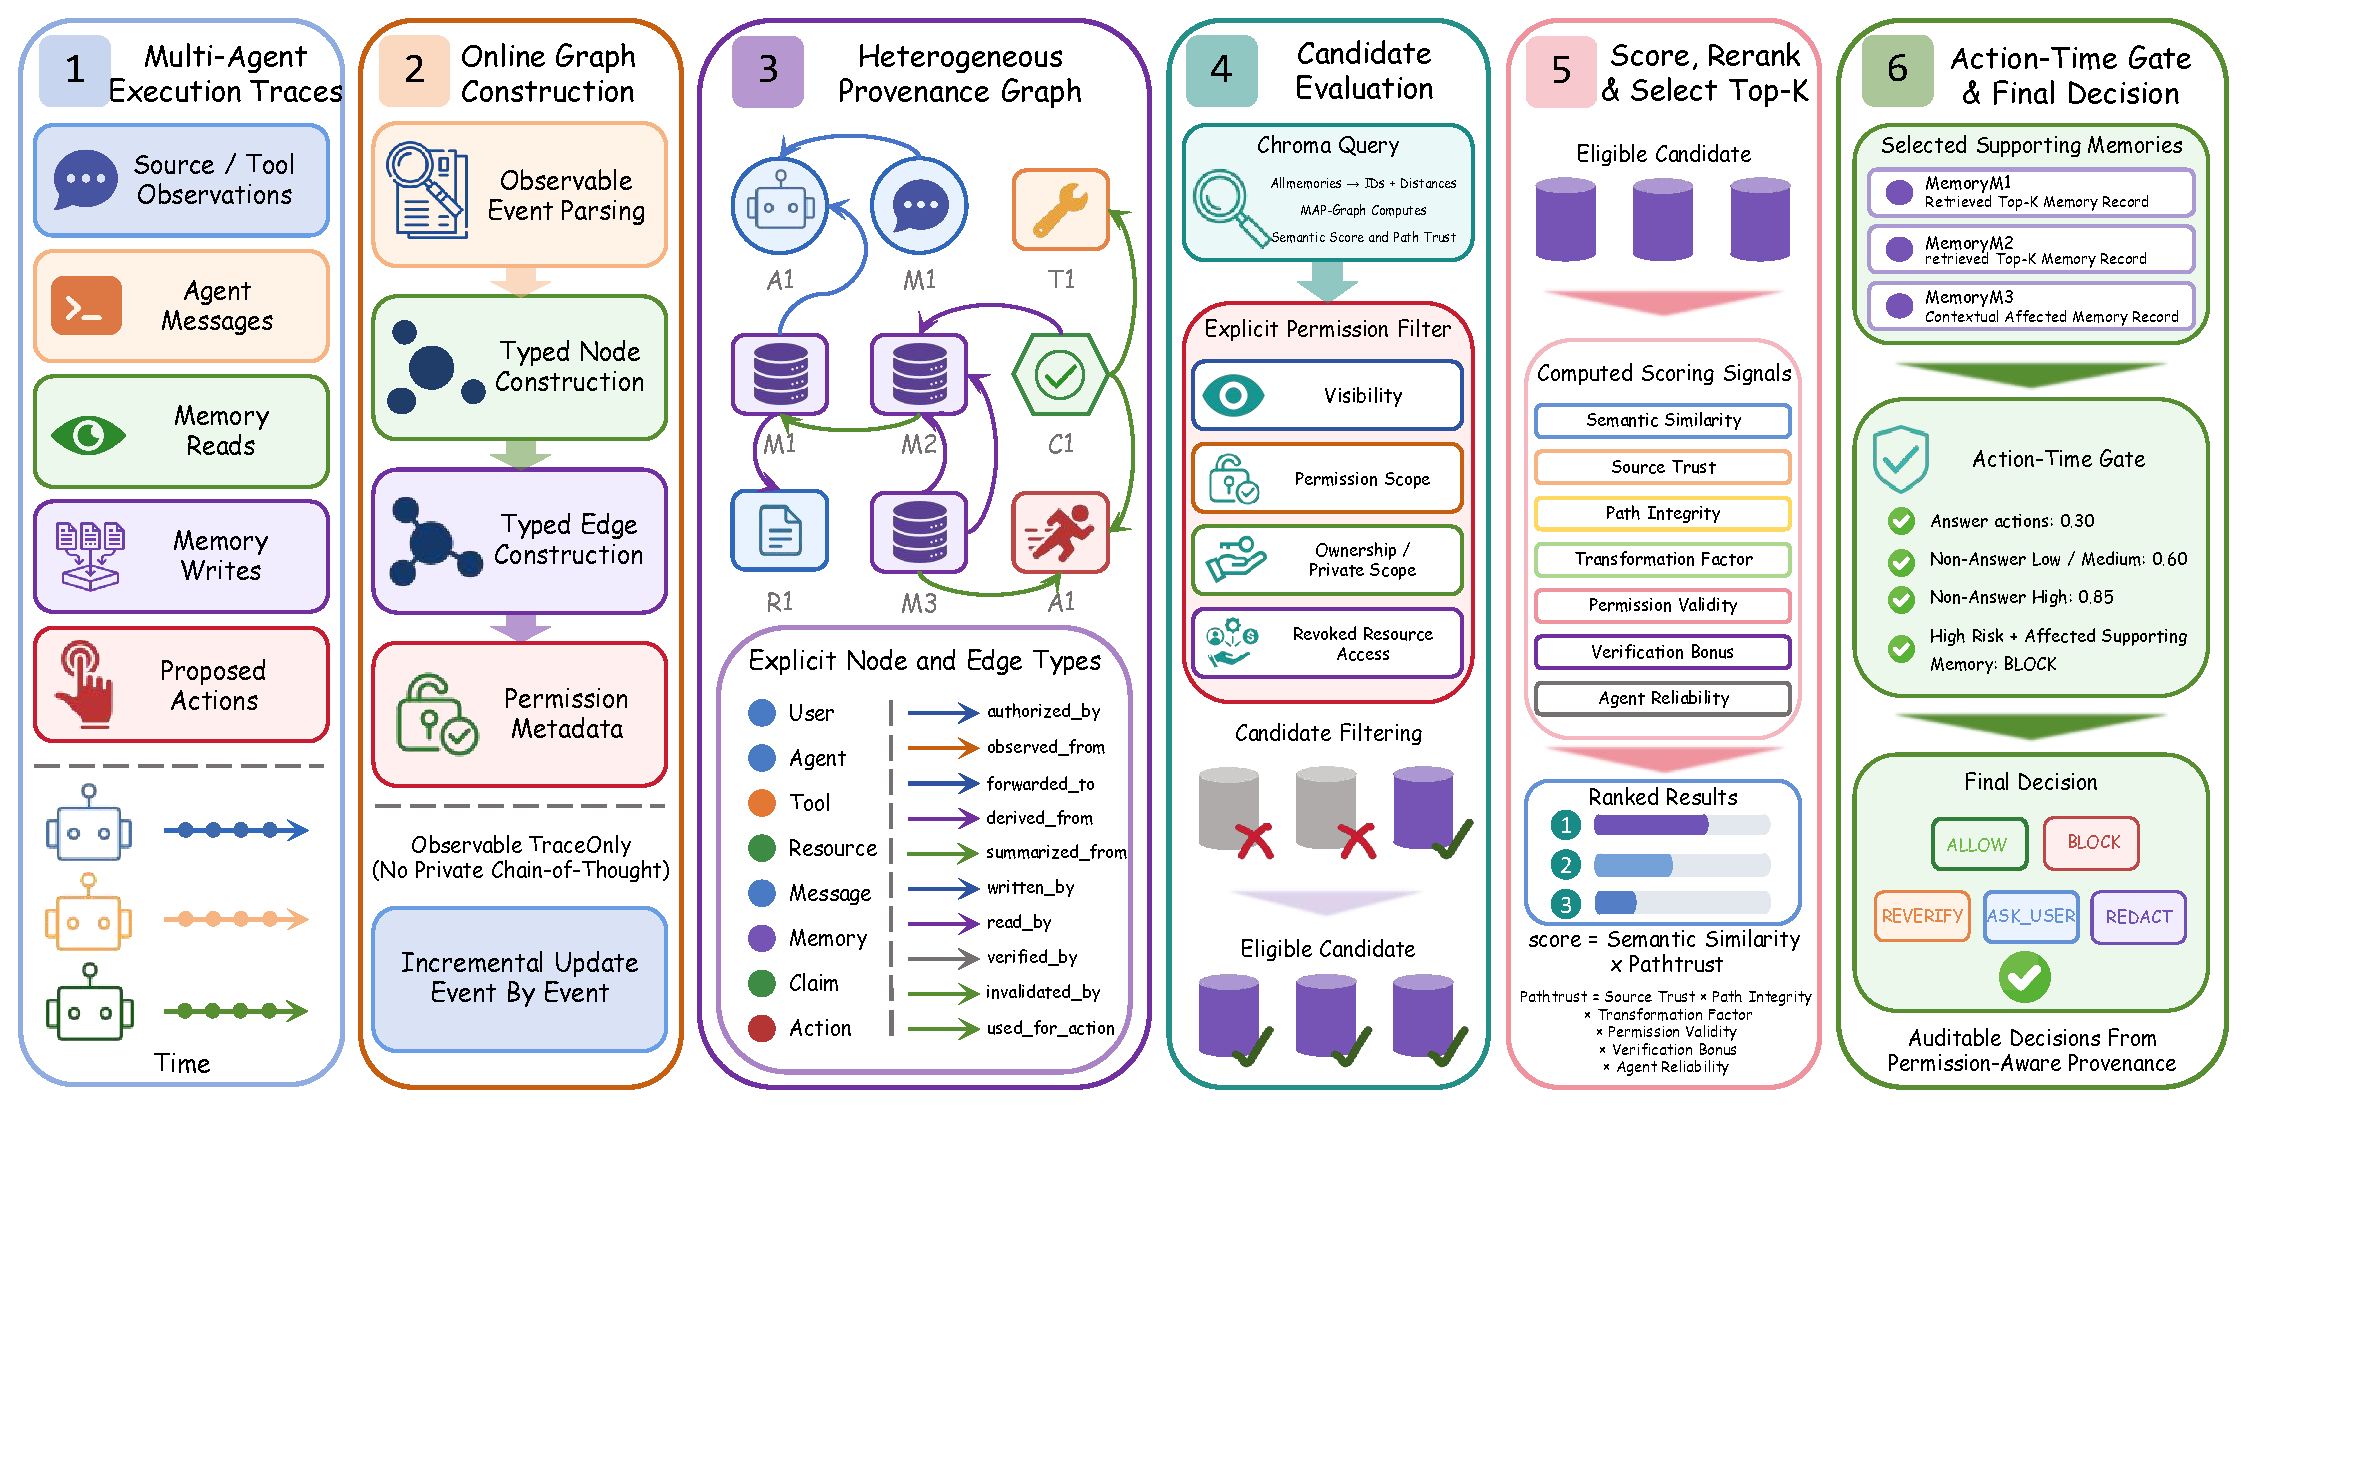
\includegraphics[
        width=0.98\textwidth,
        height=0.48\textheight,
        keepaspectratio
    ]{MAP-Graph1.pdf}
    \caption{Overview of MAP-Graph. A task-scoped typed provenance graph records memory origins and downstream dependencies. MAP-Graph combines semantic retrieval, recursive ancestry tracing, permission filtering, path-trust reranking, and risk-sensitive action gating to return \textsc{Allow}, \textsc{Block}, \textsc{Reverify}, \textsc{Redact}, or \textsc{AskUser}.}
    \label{fig:overview-map}
\end{figure*}


Language-model agents increasingly plan, use tools, and reason over long horizons~\cite{yao2023react,shinn2023reflexion}; multi-agent frameworks add role specialization and collaborative decomposition~\cite{park2023generativeagents,li2023camel,wu2024autogen,hong2024metagpt}. 
Shared memory preserves intermediate knowledge across agents and sessions~\cite{packer2023memgpt,zhong2024memorybank,wang2023longmem,zhang2025memorysurvey}. As workflows incorporate more agents, tools, and external resources, this memory becomes execution state: one agent's record can later determine another agent's answer or tool action~\cite{gao2024memorysharing,rezazadeh2025collaborativememory,zhang2025gmemory,wang2025mirix,margalit2026governed}.

This creates a failure mode that retrieval quality alone cannot diagnose. Vector retrieval can return the most relevant record~\cite{lewis2020rag,guu2020realm,karpukhin2020dpr} while remaining blind to whether that record may be read or used. Moreover, derivation can hide the relevant restriction: a summary may omit the fact that its source was private, poisoned, untrusted, or subsequently revoked. The derived memory can therefore remain highly relevant while enabling unauthorized disclosure or an unsafe downstream action~\cite{chao2026stale,dash2026memorypoisoning,pulipaka2026sleeper,wang2026mempoison}. %These failures motivate the poisoning, privacy, and revocation conditions studied here.

Existing approaches cover substantial pieces of this problem. Private/shared memory tiers enforce local access policies; graph-structured memory represents relationships~\cite{edge2024graphrag,guo2025lightrag,gutierrez2024hipporag}; and provenance models record  derivation~\cite{belhajjame2013provdm,moreau2013prov}. Recent governed shared memory further combines scoped retrieval, provenance tracking, temporal supersession, and policy propagation in a production service~\cite{margalit2026governed}. That study intentionally evaluates a live system rather than comparative action policies, leaving open how hard authorization, graded ancestry trust, and action-risk gating interact under common controlled conditions. More generally, local metadata need not expose inherited restrictions, representation alone does not determine authorization, and a retrieval-time decision need not match the risk of the eventual action. The unresolved question is therefore: \emph{how can a shared-memory system retrieve useful records while enforcing agent-, ancestry-, and action-specific admissibility?}

%But relational representation alone does not enforce authorization, and recording lineage alone does not decide whether a retrieved memory may support a particular action. The central problem is therefore not inaccurate retrieval but the conflation of two decisions: whether a memory is relevant, and whether it is admissible for use.

Our answer begins with one distinction: \emph{retrieval is not authorization}. \emph{Semantic relevance} asks whether a memory is useful for the query; \emph{provenance admissibility} asks whether the requesting agent may use it for the proposed action. 
%Admissibility is not local to a record---it depends on ownership, visibility, trust, verification, and revocation properties recorded along its provenance paths.
Operationalizing the distinction raises three challenges.
\textbf{(C1) Recursive Ancestry.} 
Admissibility may depend on multi-step derivation chains across sources and derived memories, so inspecting only a record's local metadata or immediate source is insufficient.
\textbf{(C2) Heterogeneous Constraints.} 
Permission and visibility determine whether a record is eligible for retrieval, whereas source reliability, verification, and other provenance-quality signals should grade the eligible evidence without allowing semantic similarity to override a hard access restriction. 
\textbf{(C3) Action-Dependent Admissibility.} 
Evidence sufficient for a low-risk response may be inadequate for a consequential action, so admissibility cannot be decided only once at retrieval time.

We propose \textbf{MAP-Graph}, a provenance-aware memory layer that addresses C1-C3 in sequence.
%separates semantic relevance from provenance admissibility. 
A typed execution graph records agents, sources, memories, claims, actions, and their derivations. 
Retrieval first applies permission eligibility, then combines semantic relevance with multiplicative path trust computed from recorded ancestry. Once an action is proposed, a risk-sensitive gate re-evaluates its supporting memories. Affected descendants remain marked rather than deleted, preserving evidence for audit while constraining downstream use.
%During retrieval, it first filters memories that violate permission or visibility constraints and then reranks the remaining candidates by combining semantic relevance with a multiplicative path-trust score. At the action boundary, a risk-sensitive gate re-evaluates the supporting memories according to the proposed action's risk. Memories affected by poisoned, untrusted, private, or revoked ancestry remain marked in the graph, preserving their lineage for audit while making the affected state available to downstream gating and audit. 
Figure~\ref{fig:overview-map} summarizes the workflow.

We evaluate seven baselines and six ablations on 2,700 synthetic tasks across three domains, plus three backbones on a stratified 540-task subset. MAP-Graph reaches 94.96\% task success, 72.70\% exact accuracy, and 90.22\% clean success. Removing its hard permission filter improves utility but allows every observed unauthorized read, a failure hidden by aggregate utility and leakage alone. These are single-run controlled results, not deployment-scale claims.


In summary, this paper makes the following contributions:
\begin{enumerate}
    \item We formulate provenance-aware shared-memory use as a controlled decision problem that separates semantic relevance from agent- and action-specific provenance admissibility.

    \item We propose \textbf{MAP-Graph}, which combines typed provenance representation, permission filtering, ancestry-aware trust reasoning, risk-sensitive action gating, and audit-preserving descendant marking.

    \item We provide a three-domain controlled benchmark with seven baselines, six ablations, and a stratified three-backbone comparison.
\end{enumerate}
\section{Background and Problem Formulation}
\label{sec:background-problem}

\subsection{Multi-Agent Shared Memory}
\label{sec:multi-agent-shared-memory}

We consider a set of agents $\mathcal{A}=\{a_1,\ldots,a_n\}$ collaborating on a long-horizon task. At each step an agent may observe information, call a tool, exchange messages, generate claims, or make partial decisions, producing information worth storing for later reuse. A shared memory store $\mathcal{M}$ maintains it across agents and time, with a memory entry denoted
\begin{equation}
m_i = (\mathrm{id}_i,c_i,o_i,v_i,d_i,\ell_i,\eta_i),
\label{eq:memory-entry}
\end{equation}
where $\mathrm{id}_i$ is the identifier, $c_i$ the content, $o_i$ the owner agent, $v_i$ the visibility, $d_i$ the source and parent-memory references, $\ell_i$ an optional trust label, and $\eta_i$ additional metadata. Final decisions are represented separately as Action nodes rather than as memory entries.

A score computed from $c_i$ alone cannot reveal who may read the record, which source it derives from, or whether an ancestor has been marked private, untrusted, or revoked, so the store may return an on-topic record that should not support the current action.


\subsection{Memory Provenance}
\label{sec:memory-provenance}

%Memory provenance describes a record's recorded origin and derivation history. In our implementation it is operational rather than a post-hoc log: ownership and permission scope determine candidate eligibility, while source and derivation metadata feed path trust and action gating. The benchmark supplies explicit visibility, ownership, trust, risk-tag, and revocation fields; MAP-Graph propagates referenced permission scopes at write time and recursively evaluates trust and risk signals through recorded source and parent-memory ancestry, and does not infer a universal notion of truth from unconstrained text. We represent provenance using registered entities---users, agents, tools, resources, messages, memories, claims, and proposed actions---and directed relations recording authorization, observation, forwarding, derivation, summarization, writing, reading, verification, invalidation, and action use. Section~\ref{sec:graph-schema} gives the schema implemented in the accompanying supplementary code.

Memory provenance records a record's origin and derivation. MAP-Graph uses it operationally: recorded ownership and inherited permission scope determine eligibility, while source and derivation metadata inform path trust and action gating. The benchmark supplies explicit visibility, ownership, trust, risk, and revocation fields; MAP-Graph records their lineage and does not infer a universal notion of truth from free text. Its registered entities and relations are specified in Section~\ref{sec:graph-schema} and Appendix~A.

\subsection{Provenance-Aware Retrieval Objective}
\label{sec:provenance-aware-retrieval-objective}

Let $\mathcal{M}_t$ denote the records created or seeded for task $t$, and $\mathrm{CanRead}(a,m)\in\{0,1\}$ the implemented permission check for agent $a$. For a query $q$, MAP-Graph first restricts retrieval to
\begin{equation}
\mathcal{C}(a)=\{m\in\mathcal{M}_t:\mathrm{CanRead}(a,m)=1\},
\label{eq:permission-candidates}
\end{equation}
then scores each eligible $m$ by a semantic score $s(m,q)$ from cosine distance and a path-trust value $\rho(m,a)$ computed from recorded ancestors:
\begin{equation}
\mathrm{Score}(m,q,a)=s(m,q)\,\rho(m,a).
\label{eq:implemented-retrieval-objective}
\end{equation}
The system returns the five highest-scoring candidates. This is a deterministic rule over explicit metadata, not a learned calibration of factual correctness.

The factorization is not merely notational: separating the binary gate $\mathrm{CanRead}$ from the graded factor $\rho$, and both from the content score $s$, fixes what an implementation must supply. Three requirements follow directly, restating the challenges of Section~\ref{sec:introduction} as properties of the objective rather than observations about prior systems. \textbf{Ancestry-aware evaluation (C1):} trust must be computed over the transitive recorded ancestry of $m$, while access restrictions must remain attached as memories are derived. In our implementation, a derived memory receives the intersection of its referenced scopes at write time; query-time $\mathrm{CanRead}$ then checks that stored scope and any directly referenced source. \textbf{Separation of hard and graded constraints (C2):} $\mathrm{CanRead}$ must filter the candidate set while $\rho$ multiplies the surviving scores---folding permission into $\rho$ as a large penalty would let a sufficiently similar record outrank the restriction, and folding trust into $\mathcal{C}(a)$ would discard usable evidence whose reliability is merely reduced. \textbf{A second, action-indexed decision (C3):} $\mathrm{Score}$ ranks records for a query but carries no notion of what the evidence will be used for, so admissibility for a proposed action requires a separate decision, taken after the action is known and parameterized by its risk. Sections~\ref{sec:graph-schema}--\ref{sec:trust-conflict-invalidation} present the mechanism satisfying each in turn.



\section{MAP-Graph Framework}
\label{sec:map-graph-framework}

\begin{figure*}[!t]
    \centering
    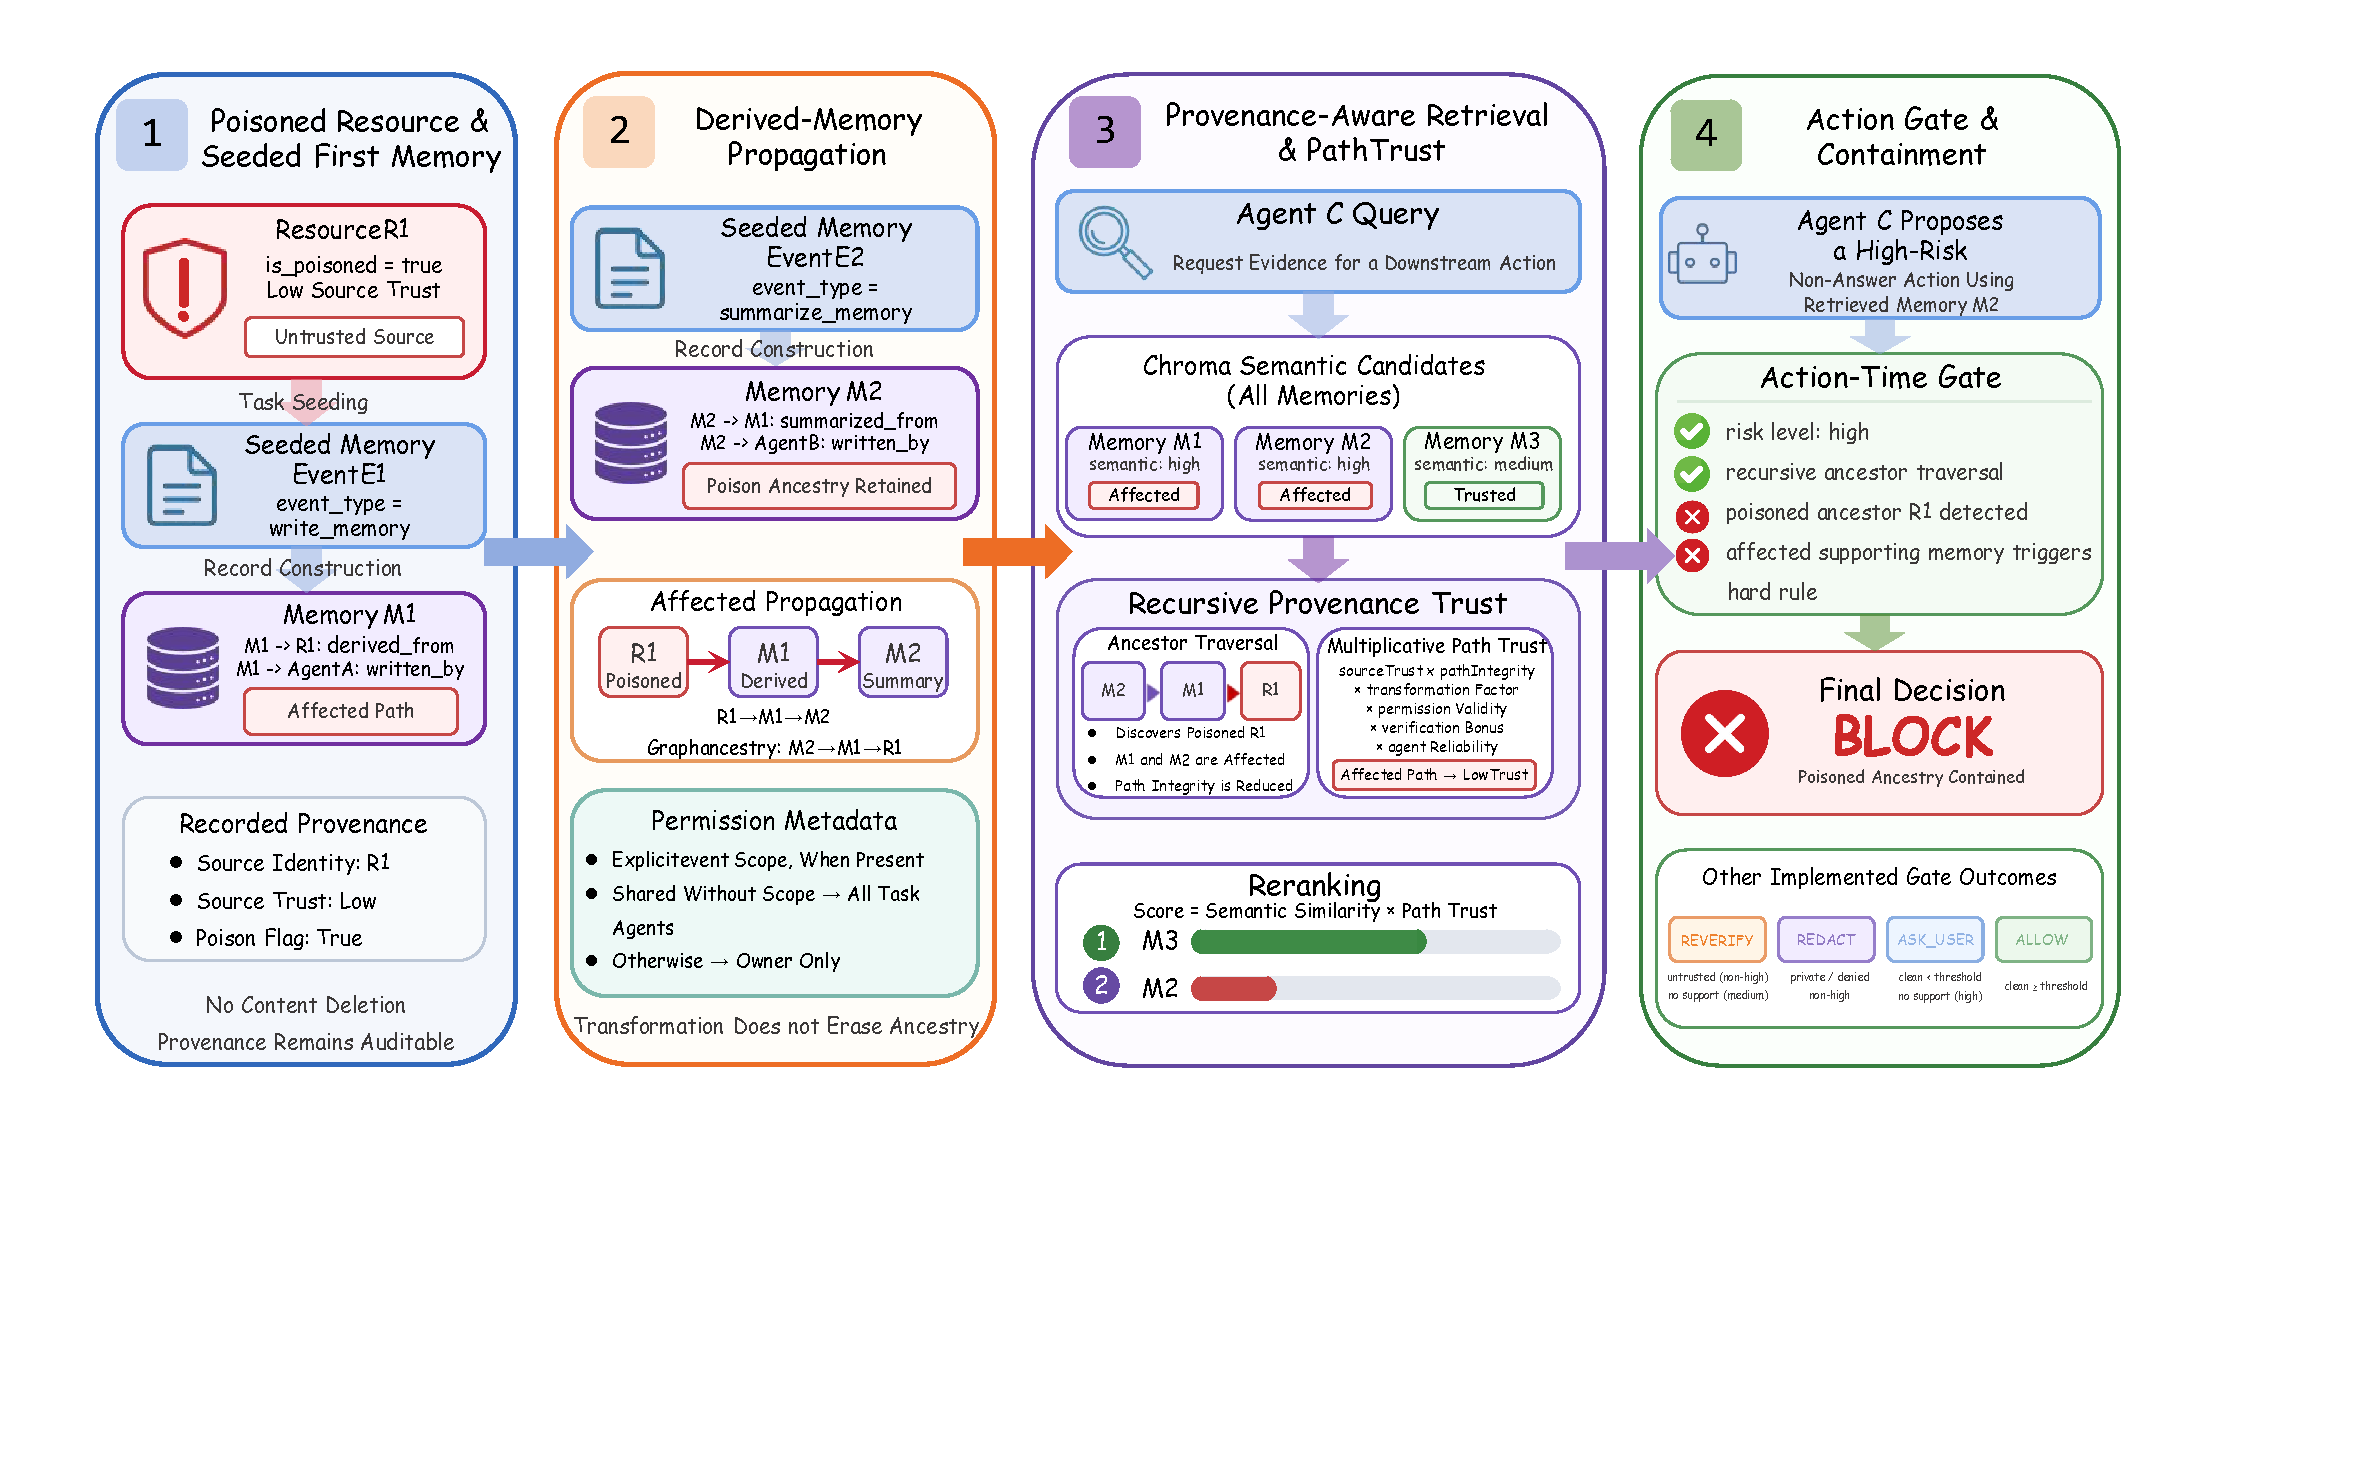
\includegraphics[
        width=0.98\textwidth,
        keepaspectratio
    ]{MAP-Graph2.pdf}
    \caption{Running example of poisoned-memory propagation and containment in MAP-Graph. A poisoned resource $R_1$ produces memory $M_1$, which is summarized into $M_2$ while retaining its provenance ancestry. During retrieval, recursive ancestry tracing identifies the poisoned source and reduces the path trust of the affected memories. When $M_2$ supports a high-risk action, the action-time gate returns \textsc{Block}, while preserving the affected lineage for audit.}
    \label{fig:running-example}
\end{figure*}

MAP-Graph is a task-scoped memory backend placed between a multi-agent workflow and its proposed action. For every task, it resets a NetworkX \texttt{MultiDiGraph}, an ephemeral Chroma collection, and the associated source and memory catalogs. The graph records observable execution lineage, while the vector collection provides semantic candidates; the two representations are coupled through common memory identifiers.

Figure~\ref{fig:running-example} illustrates the complete processing path through a poisoned-memory example. A poisoned resource $R_1$ produces memory $M_1$, which is subsequently summarized into $M_2$. Although the transformation changes the memory content, it preserves the ancestry path $M_2 \rightarrow M_1 \rightarrow R_1$. When Agent~C requests evidence for a high-risk action, recursive provenance evaluation discovers the poisoned ancestor and reduces the path trust and final ranking scores of the affected memories. If the affected memory still supports the proposed action, the action-time gate returns \textsc{Block}, while retaining the corresponding lineage for audit.

The following subsections explain this process in order: the schema and construction rules make ancestry recoverable (C1), retrieval separates hard permission filtering from graded trust reranking (C2), and the action gate re-evaluates admissibility once the proposed action is known (C3).

\subsection{Graph Schema: Registered Node and Edge Types}
\label{sec:graph-schema}

MAP-Graph represents shared memory as a heterogeneous directed provenance graph $\mathcal{G} = (\mathcal{V}, \mathcal{E}, \tau_V, \tau_E)$, where $\tau_V$ is a partial map over registered node types and $\tau_E$ assigns edge types.

The registered vocabulary has eight node types (User, Agent, Tool, Resource, Message, Memory, Claim, Action) and ten edge types: \texttt{authorized\_by}, \texttt{observed\_from}, \texttt{forwarded\_to}, \texttt{derived\_from}, \texttt{summarized\_from}, \texttt{written\_by}, \texttt{read\_by}, \texttt{verified\_by}, \texttt{invalidated\_by}, and \texttt{used\_for\_action}. The derivation edges are what make ancestry recoverable from an export alone, the precondition for the C1 evaluation in Section~\ref{sec:provenance-aware-memory-retrieval}. Task identifier, domain, step, visibility, permission scope, trust labels, and risk tags are attributes rather than node types. The graph is thus an execution-lineage representation, not a semantic knowledge graph: no generic \texttt{Contradicts}, \texttt{Updates}, or temporal-order edges are created, and no automatic open-domain conflict resolution is claimed. Per-type definitions, serialized labels, and the constants entering Equation~\ref{eq:path-trust} are in Appendix~A of the supplementary material.

\subsection{Memory Construction and Provenance Capture}
\label{sec:memory-construction-provenance-capture}

Construction uses only observable workflow state and task-provided metadata; no private chain-of-thought is required. At task initialization MAP-Graph registers the task-provided agent roles and source documents and inserts any benchmark-provided initial memory events. When an agent observes a source or tool output, the backend creates a record whose \texttt{derived\_from} field includes that identifier. When an agent writes a message-derived memory, the record inherits the identifiers of retrieved memories and visible sources, and its permission scope is the intersection of the referenced scopes; if no referenced scope exists all task agents are eligible, and if the intersection is empty access falls back to the writing agent.

Observable messages and up to three coarse Claim nodes are retained for graph inspection. The write path rejects empty text, while each non-empty write creates a distinct embedded Memory node with its own lineage. Semantically equivalent entries are not merged, and new observations do not mutate or supersede prior text; no generic supersession or conflict-resolution state machine is implemented.

An explicit \texttt{revoke\_permission} event changes the referenced source to revoked visibility, clears its permission scope, and immediately recomputes records that directly reference it or already list it as an affected ancestor, adding \texttt{invalidated\_by} edges where applicable. Other descendants detect the revoked ancestor when recursive trust is next evaluated, and task finalization marks them in the audit graph. ``Invalidation'' below therefore refers to this explicit revocation path, not a lifecycle inferred from natural-language contradictions.


\subsection{Provenance-Aware Memory Retrieval}
\label{sec:provenance-aware-memory-retrieval}

This stage implements the ancestry-closed evaluation required by C1 and the hard/graded separation required by C2. Given query $q$ from agent $a$, the backend embeds $q$, requests all task-local records, and scores each by $s(m,q)=\max(0,1-d(m,q))$ for cosine distance $d$. For each semantic candidate, MAP-Graph computes ancestry-based trust signals and applies the permission check in the same candidate loop; only eligible records enter final-score ranking. The permission check considers visibility, permission scope, the requesting agent, and directly referenced sources, and revoked sources are never readable. Trust computation recursively follows the record-level \texttt{derived\_from} list to collect source and parent-memory ancestors. This recursion feeds trust computation only; it is not a query-time $h$-hop expansion over the graph, and Claim or Resource nodes are not returned to the model.

Let $S$, $I$, $F$, $P$, $V$, and $A$ denote source trust, path integrity, transformation factor, permission validity, verification bonus, and writer reliability. Path trust is their clipped product,
\begin{equation}
\rho(m,a) = \operatorname{clip}_{[0,1]}\!\bigl(S(m)I(m)F(m)P(m,a)V(m)A(m)\bigr),
\label{eq:path-trust}
\end{equation}
and eligible records are ranked by $\mathrm{Score}(m,q,a)=s(m,q)\rho(m,a)$, of which the top five are returned. The factors have distinct inputs: $S$, $I$, and $V$ summarize recorded ancestry; $F$ follows the memory's transformation chain; $P$ is the current \texttt{CanRead} result; and $A$ is the reliability assigned to the writing agent. Thus a record with unremarkable local text can still receive low trust. In particular, $I$ is multiplied down once for each of the untrusted/poisoned, private/sensitive, and revoked categories present in the ancestry, so these category penalties compound rather than average. Revocation additionally remains a hard access or action-gate cause where the implemented rules detect it. Appendix~A of the supplementary material lists each constant.

This arrangement yields two properties. \emph{First}, ancestry-aware governance: recursive \texttt{derived\_from} traversal exposes multi-step trust and risk signals, while write-time scope intersection carries access restrictions into newly derived records. Query-time permission checks then enforce the derived record's scope and any directly referenced source; they do not independently traverse every parent record. \emph{Second}, non-substitutable constraints: permission removes candidates before ranking, so no semantic score compensates for a detected access violation, while trust only scales scores of records that already passed, so degraded but usable evidence is demoted rather than discarded. This is C2's hard/graded separation, and Section~\ref{sec:ablation} shows that collapsing it changes which failure mode appears.

\subsection{Affected Ancestry and Action-Time Gating}
\label{sec:trust-conflict-invalidation}

This stage supplies the second, action-indexed decision required by C3. The trust computation labels a memory \emph{affected} when its recursive ancestry contains an untrusted, private, or revoked item. At finalization, bookkeeping propagates this state from affected roots to predecessors connected through \texttt{derived\_from}, \texttt{summarized\_from}, or \texttt{invalidated\_by}, and affected nodes and their ancestor identifiers remain in the export. Containment therefore means restricting retrieval or action use while retaining lineage; it does not mean deleting every descendant.


Before accepting a proposed action, MAP-Graph recomputes trust for its retrieved supporting memories and for affected or permission-invalid inter-agent message memories that provide contextual support. Let $\theta$ be $0.30$ for an answer, $0.85$ for a high-risk non-answer action, and $0.60$ otherwise. The gate applies four ordered rules: (1) if a high-risk action has any affected supporting memory, return \textsc{Block}; (2) if no supporting memory survives for a medium- or high-risk action, return \textsc{Reverify}, or \textsc{AskUser} for high risk; (3) if a supporting path is private, revoked, untrusted, or permission-invalid, return \textsc{Block}, \textsc{Redact}, or \textsc{Reverify} according to risk and cause; (4) if the maximum supporting-memory trust is below $\theta$, return \textsc{Redact}, \textsc{Reverify}, or \textsc{AskUser}, and otherwise return \textsc{Allow}.

These are deterministic rules for the benchmark's decision vocabulary, an implemented policy layer rather than a proof that an allowed action is safe. Because $\theta$ and Rule~1 are indexed by the action rather than the query, the same supporting memory can be admissible for an answer and inadmissible for a high-risk external action---the behavior C3 asks for, and a distinction that a retrieval-only policy without access to the proposed action cannot express. Section~\ref{sec:main-results} reports that the residual failures remain concentrated in exactly this action-risk dimension. The export retains, per selected memory, its semantic, path-trust, and final scores, and per gate event the affected ancestors, cause, supporting identifiers, threshold, and decision; this is what makes the containment claim checkable, and Appendix~B of the supplementary material details it.

\subsection{Implementation Notes}
\label{sec:dynamic-update-complexity}

Within a task, graph, embedding, and gate state is updated incrementally; between tasks the graph and vector collection are reset, so the experiments concern within-task coordination rather than cross-session accumulation. For $M$ records, trust computation for memory $m$ is $O(D_m)$ in its reachable ancestors and ranking costs $O(M\log M)$; these are benchmark-implementation bounds, not claims of deployment-scale optimization. The backend exposes observe/write, retrieve, revoke, decide, and export; the outer workflow runs roles in fixed order and submits the proposed action to the gate. A restrictive backend decision is never relaxed: a conservative agent proposal stands when the backend returns \textsc{Allow}. Appendix~B gives the operation semantics.

\section{Experiments}
\label{sec:experimental-setup}

We evaluate MAP-Graph as an implemented safety layer for shared multi-agent memory along three questions: \textbf{RQ1 (utility)}, whether task success and exact decisions improve without sacrificing clean-task utility; \textbf{RQ2 (safety)}, whether poisoned, private, and revoked memories cross read or action boundaries; and \textbf{RQ3 (robustness)}, whether the effects persist across domains, scenarios, and model backbones. Section~\ref{sec:ablation} probes components associated with C1--C3.

\begin{table*}[!t]
\centering
{\small
\setlength{\tabcolsep}{3pt}
\begin{tabular}{@{}lrrrrrrrr@{}}
\toprule
Method & TSR $\uparrow$ & Acc $\uparrow$ & Clean $\uparrow$ & Unsafe $\downarrow$ & ASR $\downarrow$ & Leak. $\downarrow$ & UAcc $\downarrow$ & Revok. $\downarrow$ \\
\midrule
B0: No Memory                       & 65.52 & 40.37 & 84.33 & 28.81 & 33.56 & 32.44 & N/A & 39.78 \\
B1: Shared Vector Memory            & 67.30 & 40.93 & 88.78 & 28.37 & 30.89 & 20.89 & 100.00 & 47.56 \\
B2: Isolated Vector Memory          & 69.15 & 41.63 & 86.00 & 25.59 & 30.00 & 18.00 & N/A & 40.00 \\
B3: Adapted G-Memory                & 66.00 & 37.63 & 86.89 & 29.19 & 33.56 & 32.22 & 100.00 & 38.00 \\
B4: Adapted Collaborative Memory    & 69.07 & 41.85 & 88.67 & 26.63 & 33.11 & 19.33 & 43.08 & 39.78 \\
B5: Adapted MemLineage              & 74.37 & 51.07 & 88.11 & 21.19 & 22.22 & 23.33 & 100.00 & 23.78 \\
B6: Flat Provenance                 & 74.67 & 46.41 & 88.00 & 20.81 & 36.44 & 20.44 & 43.08 & 39.33 \\
\midrule
MAP-Graph                           & 94.96 & 72.70 & 90.22 & 1.52 & 0.00 & 0.00 & 0.00 & 0.00 \\
\bottomrule
\end{tabular}
}
\caption{Main results over 2,700 tasks per method (percent). UAcc is conditional unauthorized access; N/A means no observed attempt. B3--B5 are benchmark adaptations, and B6 is the flat-metadata control. Additional diagnostic rates are reported in the supplementary material.}
\label{tab:main-results}
\end{table*}

\subsection{Benchmark and Protocol}
\label{sec:task-domains}

The controlled synthetic benchmark contains 2,700 tasks generated with seed 42 and split evenly across corporate workflow, software engineering, and research assistance. Each domain contributes 150 tasks to each of six groups: clean utility, poisoned propagation, private leakage, permission revocation, action-risk sensitivity, and clean compression/overhead. Every domain--group cell contains 15 semantic families with 10 variants; oracle labels total 960 \textsc{Allow}, 1,140 \textsc{Block}, 210 \textsc{Reverify}, and 390 \textsc{Redact}.

Each task provides sources, memory and tool events, visibility, four fixed-order roles, and a risk-labelled proposed action; no external side effect is executed. Methods receive identical inputs and differ only in memory retrieval and access policy. Before execution, a sanitizer removes the oracle, evaluator rationale, and experiment/family/variant identifiers while retaining the provenance and policy fields under study. One run per method over the same task order yields 21,600 decision logs. The 95\% intervals use 2,000 cluster-bootstrap samples over semantic families and quantify within-run case variation, not inference nondeterminism. Supplementary Appendix~C gives the construction and sanitizer.

\subsection{Baselines}
\label{sec:baselines}

Seven baselines run behind the same workflow and memory interface. \textbf{B0 (No Memory)} keeps only the current conversation. \textbf{B1 (Shared Vector Memory)} pools all records in one Chroma collection and retrieves the five most similar; \textbf{B2 (Isolated Vector Memory)} uses the same retrieval with a per-agent store. \textbf{B3 (Adapted G-Memory)} converts observable traces into trajectories over query, interaction, and insight graphs~\cite{zhang2025gmemory}. \textbf{B4 (Adapted Collaborative Memory)} assigns records to private or shared tiers from visibility metadata and applies access-control filtering to similarity candidates before final ranking and top-$k$ return~\cite{rezazadeh2025collaborativememory}. \textbf{B5 (Adapted MemLineage)} records derivation ancestors and applies a lineage-sensitive check before high-risk actions, without permission filtering~\cite{ouyang2026memlineage}. \textbf{B6 (Flat Provenance)} is a controlled local-metadata baseline. It retains the direct visibility, owner, permission scope, source trust, private/revoked/poisoned state, and action risk available to MAP-Graph, but constructs no provenance graph, never traverses parent records, and performs no recursive ancestry or path-trust propagation. Its retrieval filter and multi-outcome action check inspect only the current memory's stored metadata. B6 therefore isolates recursive graph ancestry from the benefit of having rich per-record governance fields.

B3 has no permission-aware filtering, trust propagation, or gate; B4 provides access-controlled retrieval only; B5 adds a high-risk lineage check without permission-aware retrieval or multi-agent trust decay; and B6 inspects local metadata only. B6 is a controlled comparator rather than an adaptation of an external system. Thus none combines hard filtering, recursive graded path-trust reranking, and ancestry-aware gating. We describe B3--B5 as benchmark adaptations rather than reimplementations; Appendix~D records the full configurations and disabled components.

\subsection{Metrics and Implementation}
\label{sec:evaluation-metrics}

\textbf{Acc} is exact decision accuracy; \textbf{TSR} requires \textsc{Allow} on allowed cases and credits any safe intervention otherwise. \textbf{Clean} is the \textsc{Allow} rate in Exp-1/6. \textbf{Unsafe}/\textbf{ASR} are impermissible execution rates overall/in the poisoned-memory group. \textbf{Leakage} counts private cases ending in \textsc{Allow} or exposing the canary; \textbf{Revocation}, \textsc{Allow} after withdrawal. \textbf{UAcc} is successful/observed unauthorized reads (undefined with no attempt). Appendix~E gives formulas.

All methods use the AutoGen OpenAI-compatible client with Qwen2.5-7B-Instruct at temperature 0, one interaction round, and at most five retrieved items; embedding-based methods use normalized BAAI/bge-small-en-v1.5 with $k=5$. MAP-Graph applies permission filtering, multiplicative path trust, affected-state propagation, an action-time decision over retrieved and contextual supporting memories, with thresholds 0.30 for answers, 0.60 for low/medium-risk actions, and 0.85 for high-risk actions. Token usage and graph size are retained as diagnostics in Appendix~F.

\begin{table*}[!t]
\centering
{\small
\setlength{\tabcolsep}{4.2pt}
\begin{tabular}{@{}lrrrrrrr@{}}
\toprule
Variant & TSR $\uparrow$ & Acc $\uparrow$ & Clean $\uparrow$ & Unsafe $\downarrow$ & ASR $\downarrow$ & UAcc $\downarrow$ & Rev. $\downarrow$ \\
\midrule
Full MAP-Graph       & 94.96 & 72.70 & 90.22 & 1.52  & 0.00  & 0.00   & 0.00 \\
Compressed graph     & 94.33 & 71.93 & 89.22 & 1.56  & 0.00  & 0.00   & 0.00 \\
No action-time gate  & 69.44 & 42.63 & 90.00 & 27.00 & 34.89 & 0.00   & 35.11 \\
No containment       & 70.67 & 43.15 & 89.22 & 25.41 & 32.89 & 0.00   & 39.78 \\
No permission filter & 96.00 & 78.63 & 89.44 & 0.04  & 0.22  & 100.00 & 0.00 \\
No provenance stack  & 67.89 & 41.89 & 89.00 & 27.89 & 29.33 & 100.00 & 46.67 \\
No trust propagation & 87.37 & 56.44 & 88.78 & 8.56  & 0.00  & 0.00   & 0.00 \\
\bottomrule
\end{tabular}
}
\caption{Single-run ablations over 2,700 tasks per variant (percent). Clean is clean-task TSR; UAcc is conditional unauthorized access. Full diagnostics appear in the supplementary material.}
\label{tab:ablation-results}
\end{table*}

\subsection{Main Results}
\label{sec:main-results}

Table~\ref{tab:main-results} reports the aggregate utility and safety metrics for all eight methods.

\paragraph{Overall utility.}
MAP-Graph reaches 94.96\% TSR and 72.70\% exact accuracy. Relative to B6, the strongest TSR baseline, the TSR gain is 20.30 percentage points; relative to B5, the strongest exact-accuracy baseline, the accuracy gain is 21.63 points. MAP-Graph achieves 90.22\% clean TSR, the mean of its Exp-1 and Exp-6 results, so the aggregate safety gain is not produced by simply rejecting most clean requests.

\paragraph{Safety outcomes.}
MAP-Graph reduces ASR, measured leakage, and revocation violation to 0\%, with 1.52\% unsafe actions versus the strongest baseline value of 20.81\% (B6). It also blocks every observed unauthorized read; B4 and B6 permit 43.08\%, while B1, B3, and B5 permit all observed attempts. These are conditional rates: 100\% means every observed attempt succeeded, not that every read was unauthorized. Supplementary Appendix~F reports block rates, token use, and error counts.

\paragraph{Scenario-level behavior.}
MAP-Graph's largest gains occur when decisions depend on memory state: poisoned ancestry, private ownership, and permission withdrawal, for which it blocks all 450 revoked cases. In the action-risk group, however, 41 of 450 decisions remain impermissible \textsc{Allow} outcomes (9.11\%), identifying the action-time threshold as the main remaining weakness. Scenario, domain, and structural-contamination results are in Appendix~F.

\paragraph{Scope and limitations.}
The benchmark is synthetic and templated, actions are simulated, and every task uses one four-agent round. B3 alone retains up to 512 run-scoped trajectories and may be order-sensitive. One temperature-zero run does not estimate inference nondeterminism, and 3.89--9.08\% of outer calls reach the 2,048-token cap. TSR must be read with Acc because it credits any safe intervention. Finally, B3--B5 are core-mechanism adaptations, not complete reproductions.

\subsection{Backbone Transfer}
\label{sec:backbone-transfer}

We select a fixed 20\% subset (540 tasks; seed 2027), jointly stratified by domain, experiment group, and oracle label. It contains 180 tasks per domain, 90 per group, and all four labels. B1, B4--B6, and MAP-Graph use identical settings with Qwen2.5-7B-Instruct, GLM-4-9B-0414, and Llama-3.1-8B-Instruct. Qwen results are extracted from full runs; GLM and Llama are single subset runs. Only the generation backbone changes, yielding 2,700 decisions per backbone.

\begin{table*}[!t]
\centering
{\small
\setlength{\tabcolsep}{2.7pt}
\begin{tabular}{@{}lrrrrrrrrr@{}}
\toprule
Method &
\multicolumn{3}{c}{Qwen2.5-7B} &
\multicolumn{3}{c}{GLM-4-9B} &
\multicolumn{3}{c}{Llama-3.1-8B} \\
\cmidrule(lr){2-4}\cmidrule(lr){5-7}\cmidrule(l){8-10}
& TSR $\uparrow$ & Acc $\uparrow$ & Unsafe $\downarrow$
& TSR $\uparrow$ & Acc $\uparrow$ & Unsafe $\downarrow$
& TSR $\uparrow$ & Acc $\uparrow$ & Unsafe $\downarrow$ \\
\midrule
B1        & 65.19 & 40.00 & 29.07 & 86.48 & 40.93 & 3.52 & 88.89 & 59.07 & 6.11 \\
B4        & 67.22 & 40.74 & 26.67 & 85.37 & 42.59 & 4.26 & 89.81 & 61.30 & 5.93 \\
B5        & 71.11 & 49.26 & 24.07 & 87.04 & 72.59 & 3.15 & 90.93 & 70.93 & 3.89 \\
B6        & 70.93 & 43.52 & 22.59 & 88.89 & 47.96 & 1.30 & 93.52 & 65.00 & 2.59 \\
MAP-Graph & 93.33 & 72.59 & 2.04  & 86.30 & 74.81 & 0.19 & 94.26 & 80.00 & 1.30 \\
\bottomrule
\end{tabular}
}
\caption{Backbone transfer on the same stratified 540-task subset (percent). Boundary-specific diagnostics are reported in the supplementary material.}
\label{tab:backbone-transfer}
\end{table*}

Across all three backbones, MAP-Graph has the highest exact accuracy and lowest unsafe rate. It also leads TSR on Qwen and Llama; on GLM its 86.30\% trails B6's 88.89\%, exposing a utility--safety trade-off. Boundary diagnostics further show zero observed unauthorized access for MAP-Graph on every backbone (Appendix~F). Because these are single-run point estimates, they support transfer of exact decision quality and access enforcement, not backbone-invariant utility or run-to-run stability.

\subsection{Ablation Results}
\label{sec:ablation}

We evaluate six variants on the same 2,700 tasks. No gate disables only the final action gate; no containment disables affected-state enforcement and descendant marking; no permission removes \texttt{CanRead}; and no trust disables propagation and reranking. No provenance stack is a retrieval-only control disabling the graph, permission, trust and reranking, contextual support, gate, and containment. Compressed retains all decision mechanisms but exports a reduced source--memory--action graph.

Three conclusions follow. \textbf{Gate and containment (C3):} removing either sharply increases ASR, revoked-memory use, and unsafe actions while clean TSR changes by at most one point. \textbf{Trust propagation (graded C2):} removing path trust leaves the permission and gate rules active but lowers TSR by 7.59 points and raises Unsafe from 1.52\% to 8.56\%. Thus the gap measures propagation and trust-aware reranking on top of permission filtering and gating. \textbf{Compression:} TSR changes by 0.63 points while the export shrinks from 39.74 to 24.66 nodes and 246.78 to 70.68 edges.

\paragraph{Utility gains can mask an access-control failure.}
Without the permission filter, TSR rises from 94.96\% to 96.00\% and Acc from 72.70\% to 78.63\%, yet UAcc rises from 0\% to 100\%. Restricted records improve retrieved context, while the downstream gate still suppresses most prohibited use; it cannot undo an unauthorized read. Hence governed-memory evaluation must instrument the access boundary rather than rely only on utility and end-to-end leakage.

\section{Related Work}
\label{sec:related-work}

\noindent\textbf{Memory in LLM agents.} Agent-memory systems support persistence, sharing, collaboration, governance, and structure~\cite{packer2023memgpt,zhong2024memorybank,wang2023longmem,zhang2025memorysurvey,gao2024memorysharing,wang2025mirix,margalit2026governed}. The closest systems motivate complementary mechanisms: G-Memory's trajectory graphs~\cite{zhang2025gmemory}, Collaborative Memory's private/shared tiers~\cite{rezazadeh2025collaborativememory}, and MemLineage's derivation enforcement~\cite{ouyang2026memlineage}. MAP-Graph does not subsume them; it combines task-local permission filtering, multiplicative ancestry scoring, affected-state audit metadata, and action-time gating.

\smallskip
\noindent\textbf{Orchestration and retrieval.} Agent and multi-agent frameworks organize roles and execution~\cite{yao2023react,shinn2023reflexion,li2023camel,wu2024autogen,hong2024metagpt}; RAG and graph retrieval improve grounding and multi-hop coverage~\cite{lewis2020rag,guu2020realm,karpukhin2020dpr,edge2024graphrag,guo2025lightrag,gutierrez2024hipporag,qian2025memorag}. MAP-Graph instead records execution lineage to govern admissibility and audit.

\smallskip
\noindent\textbf{Provenance and evidence tracing.} W3C PROV formalizes derivation relations~\cite{belhajjame2013provdm,moreau2013prov}, while long-context utilization, stale-memory, and poisoning studies expose distinct failures in evidence use~\cite{liu2024lost,chao2026stale,dash2026memorypoisoning,pulipaka2026sleeper,zhang2026memmorph,wang2026mempoison}. MAP-Graph uses lineage and access metadata operationally for retrieval and gating, not automatic truth maintenance.

\section{Conclusion}
\label{sec:conclusion}

MAP-Graph separates semantic relevance from provenance admissibility through recursive ancestry, permission filtering, path-trust reranking, and action-time gating. In the single-run 2,700-task benchmark it reaches 94.96\% TSR and 72.70\% Acc, with 0\% observed ASR, leakage, and revocation violation. On the 540-task subset it retains the highest Acc across Qwen, GLM, and Llama, although utility varies by backbone. These controlled results show that provenance can govern retrieval and actions rather than serve only as post-hoc metadata. Future work should test repeated, less templated, cross-session, and deployment-scale settings.


\bibliography{references}


\end{document}
